\section{Method}
\label{sec:method}

\begin{figure*}[t]
    \centering
    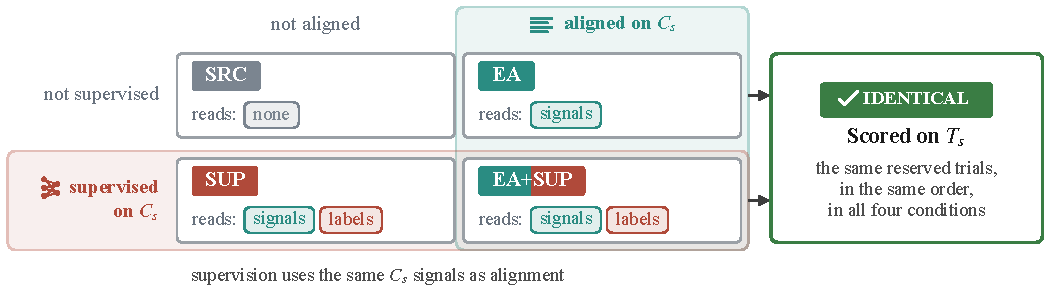
\includegraphics[width=\textwidth]{figures/figure2.pdf}
    \caption{The four conditions as a $2\times2$ over the two procedures, with what each reads from the held-out subject's available half $C_s$. Supervised training reads those trials' signals as well as their labels, so the procedures overlap. Everything else is held fixed, as Section~\ref{sec:controls} sets out, and all four are scored on the same reserved trials in the same order.}
    \label{fig:grid}
\end{figure*}

\subsection{Conditions}
We evaluate leave-one-subject-out on the three motor-imagery datasets of Table~\ref{tab:datasets}. Each held-out subject's trials are divided once, stratified by class under a per-subject seed, into an available half $C_s$ and a reserved half $T_s$ (Fig.~\ref{fig:overview}b); that 50/50 division is the declared target-data budget, no condition can change it, and $T_s$ is only ever scored.

Figure~\ref{fig:grid} shows the design. Both procedures read $C_s$: supervised training on it consumes those trials' signals as well as their labels. Each axis of the grid names a procedure applied to those trials, and both axes have the same access to them.

Alignment uses signals and no labels. Euclidean Alignment~\cite{he2020transfer} whitens a subject's trials by $\bar{R}^{-1/2}$, where $\bar{R}$ is the mean over that subject's trials of the sample spatial covariance $XX^{\top}/T$, computed on the band-passed epochs with no shrinkage and inverted through an eigendecomposition whose eigenvalues are floored at $10^{-10}$ to keep a rank-deficient epoch from blowing up. Source subjects are whitened by a reference estimated from all of their trials, which is legitimate because all of them are available. The held-out subject's reference is estimated from $C_s$ alone and then frozen; $T_s$ is transformed by it but never contributes to it. The switch also changes how every source subject is preprocessed, so the measured effect is that of the whole alignment pipeline. Target supervision adds $C_s$ to the training set with its labels attached.

The four conditions are neither procedure (SRC), alignment only (EA), supervision only (SUP), and both (EA+SUP). Two further arms sit off the grid, each changing a third thing: SEL picks the checkpoint on $C_s$ rather than the source validation set, leaving training set, initialization and trajectory unchanged but swapping a selection set of very different size; POOL adds $C_s$ to the same scaler's fit set. $T_s$ enters no scaler.

\begin{table}[b]
\centering
\caption{The three motor-imagery datasets. Trials per half is the declared target-data budget: each held-out subject is cut once into an available half $C_s$ and a reserved test half $T_s$ of that size. Chance is given in parentheses; it differs across the datasets, so accuracies are not comparable between them.}
\label{tab:datasets}
\small
\setlength{\tabcolsep}{4pt}
\begin{tabular}{@{}lcccc@{}}
\toprule
& Subjects & Channels & Classes & Trials/half \\
\midrule
BCI IV 2a \cite{tangermann2012bcicompiv} & 9 & 22 & 4 ($0.25$) & 288 \\
BNCI2014-002 \cite{steyrl2016bnci} & 14 & 15 & 2 ($0.50$) & 80 \\
PhysionetMI \cite{schalk2004bci2000,goldberger2000physionet} & 105 & 64 & 4 ($0.25$) & 45 \\
\bottomrule
\end{tabular}
\end{table}


\subsection{Controlled variables}
\label{sec:controls}
Three quantities are pinned exactly:
\begin{itemize}[nosep,leftmargin=1.2em]
\item the source partition: the stratified 80/20 split supplying training and selection data is derived from the outer pool alone and is the same index set in all four conditions, and validation is source-only throughout, so target trials never reach the selection set;
\item the epoch: every condition draws, with replacement, as many samples per epoch as the source training set holds (3686, 1664 and 7486);
\item the scored object: $T_s$ is identical across conditions, trial for trial.
\end{itemize}
A fourth, the target sampling rate, is fixed in expectation: a plain shuffled loader over the same pool would give the target 7.2\%, 4.6\% and 0.6\% of a batch, a 12-fold range set by cohort size. The supervised arms therefore use a weighted sampler with a declared expected share of 0.10, realized at 0.096--0.109.

Two quantities this does not equalize, and we report both. Because the epoch is a fixed total, a supervised arm draws 10\% fewer source samples per epoch than SRC; and because each arm early-stops on its own curve, realized updates differ: taking fold-averaged totals per arm and dividing the spread by the smallest, by 10\% on 2a, 3\% on PhysionetMI and 23\% on BNCI2014-002. Exposure is the sharper problem: a declared share $w$ implies $wS/|C_s|$ expected draws of each target trial per epoch, which is 1.3, 2.1 and 16.6 here, since $|C_s|$ differs 6.4-fold. Matching repetition instead would need shares of 0.156, 0.096 and 0.012; matching both would need source exposure to vary 13-fold. Any such comparison fixes two of these three and lets the third move, which is why we vary $|C_s|$ directly in Section~\ref{sec:results}.

An earlier version of this study enforced none of these controls, and replaying it gives the pattern of Fig.~\ref{fig:overview}a: a supervised arm on a re-drawn source partition with target trials in its validation set and batch shares of 6.1, 3.8 and 0.5\%, which its cross-dataset ordering followed; a selection arm with 25\% more source trials than its reference; and a whitener fitted on $C_s \cup T_s$. None shows in a results table, so a script checks the controls against the realized indices before any run.

\subsection{Aggregation unit}
\label{sec:aggregation}
A cross-subject spread is read as between-subject heterogeneity, which requires the aggregation unit to be the subject. We test that with a control that retrains nothing: the per-trial predictions on $T_s$ are held fixed and only the grouping changes, first by true subject, then into random groups of the same sizes, 2000 times, on SRC and SUP. Trial-weighted accuracy is identical either way, and subjects contribute equal trial counts on 2a and BNCI2014-002 and near-equal ones on PhysionetMI (45 for 104 subjects, 44 for one), so the subject macro-average and the trial-weighted average coincide up to that single trial and any difference in spread belongs to the grouping alone. The null is not a new phenomenon: drawing $m$ of $M$ correctness records without replacement gives group means of variance $(1-m/M)S^2/m$, which our resampled null reproduces. What it adds is how much of a reported spread that accounts for, where $m$ ranges from 45 to 288.

\subsection{Statistics}
\label{sec:stats}
Each subject contributes one number per condition, averaged over three runs. Those runs vary the target split and the initialization together, so they estimate neither alone; within a run all conditions share both, which is what the pairing requires. Differences are paired within subject and resampled over subjects, with one set of bootstrap indices drawn per dataset and reused for every condition ($10^4$ replicates, percentile intervals~\cite{efron1994bootstrap}). $p$-values come from a two-sided sign-flip permutation test~\cite{winkler2014permutation} over the five conditions of a dataset, Holm-corrected~\cite{holm1979simple} within that family, with a paired $t$-test as a sensitivity check. That test saturates on a small cohort: on nine subjects it cannot return less than $2/2^{9}=0.0039$, so we report the number of subjects helped beside it. Spread comparisons are ratios of standard deviations, so every factor quoted below is on that scale.

Because leave-one-subject-out folds share most of their training pool, the subjects are not independent replicates~\cite{nadeau2003inference}, and with nine of them on 2a the reference distribution is coarse. We therefore read a Holm-adjusted $p$ below 0.05 as a difference resolved by this repetition structure (these subjects, these runs, this training policy) and not as inference about a subject population, and we use that as the single rule for which differences we state. Intervals give magnitude only: they carry no multiplicity adjustment, and in a Gaussian simulation at $n=9$ our percentile intervals covered 89\% rather than 95\%, so an interval excluding zero beside a non-significant adjusted $p$ is not evidence of an effect.
